\documentclass[english]{article}
\usepackage[T1]{fontenc}
\usepackage[latin9]{inputenc}
\usepackage{geometry}
\geometry{verbose,tmargin=1cm,bmargin=1cm,lmargin=1in,rmargin=1in,headheight=1cm,headsep=1cm,footskip=1cm}
\pagestyle{empty}
\setcounter{secnumdepth}{2}
\setcounter{tocdepth}{2}
\usepackage{amstext}
\usepackage{graphicx}
\usepackage{babel}
\begin{document}
\begin{center}

{\huge Instructions: The Rook's Walk Puzzle}{\huge \par}

\end{center}\rule[0.5ex]{1\columnwidth}{1pt}

\noindent To solve the puzzle
\begin{enumerate}
\item Place the rook in the grid, move it $N$ square in some direction and write the number $N$ where it lands.
\item 
Next choose a \textbf{different} direction and repeat until the rook arrives back where it started.
\item 
The numbers written in any given row or column must be different and the sums of the rows and columns must match the corresponding numbers on the boundary.
\end{enumerate}
Note: The rook should land on or pass through every white square. Some numbers are provided as hints!
\begin{center}
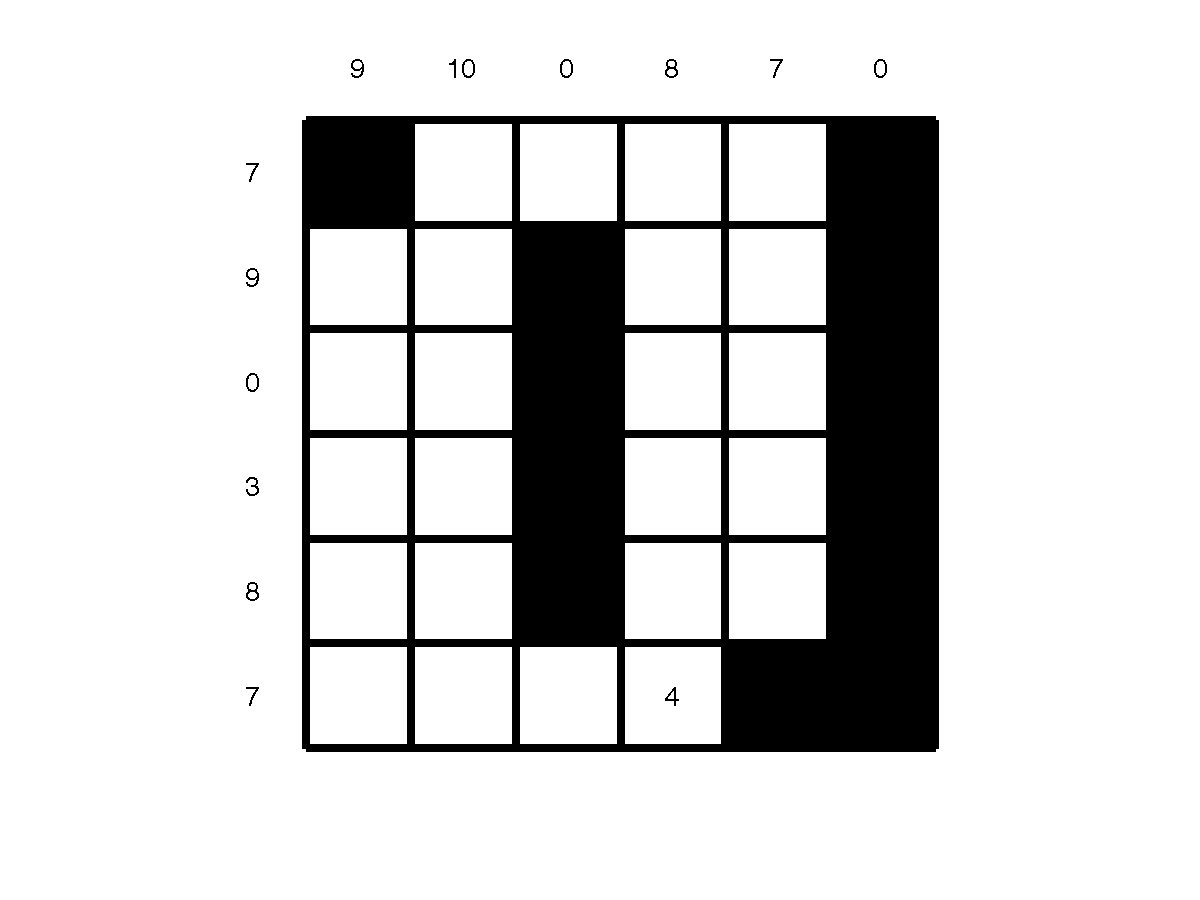
\includegraphics[scale=0.6]{medium}
\end{center}
\begin{center}
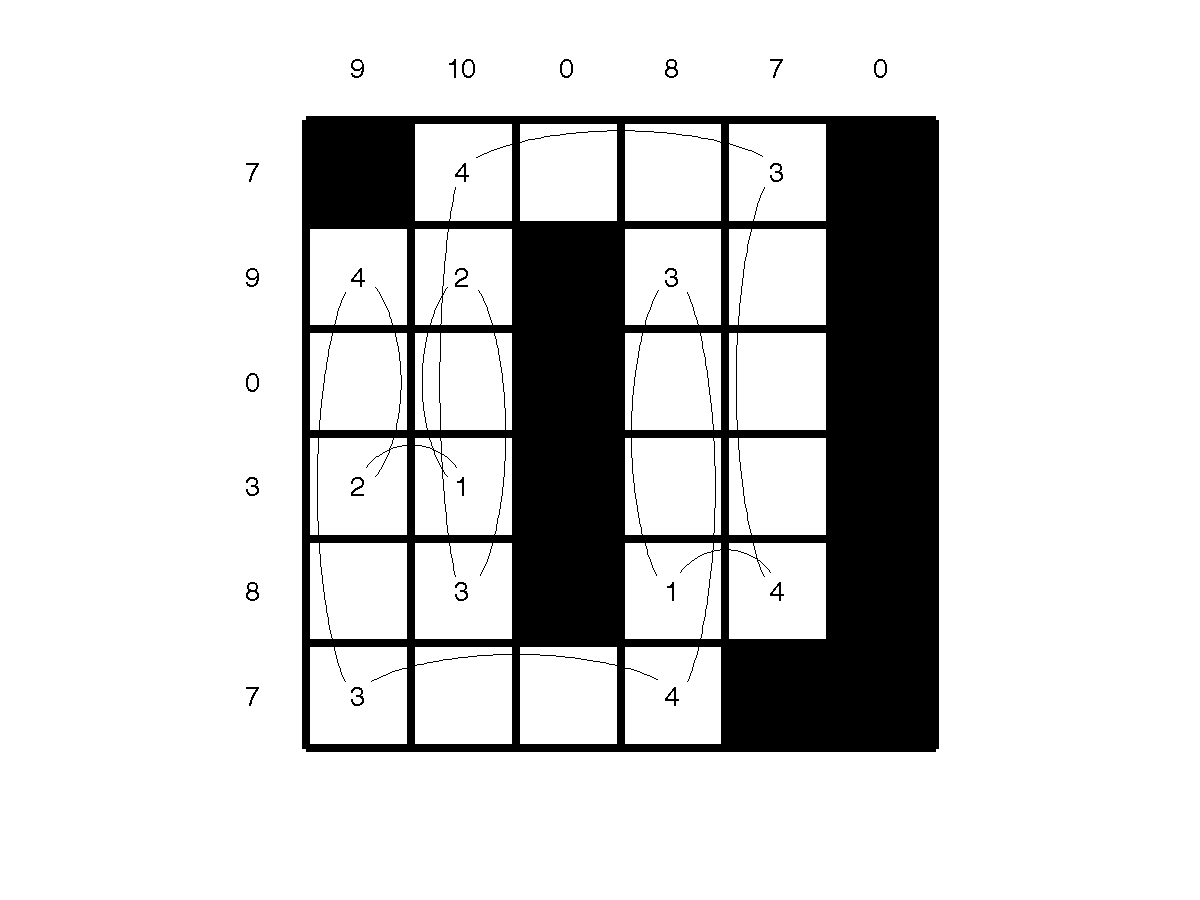
\includegraphics[scale=0.6]{mediumsoln}
\end{center}
\end{document}
